\section[Angeluaren egiaztapena]{Angeluaren egiaztapena eta seinaleen iragazpena}\label{sec:angelu-egiaztapena}
Kalkulatutako angelua egiaztatzeko, nodoaren logeko $\theta$ balioa Gazeboko \texttt{/gz\_pose} datuetatik lortutako orientazioarekin alderatu dugu. Zuzenetan, batez besteko aldea $-0{,}4^\circ$ izan da, eta desbideratze estandarra $2{,}1^\circ$. Emaitza horrek erakusten du erregresioak paretaren norabidea behar adinako zehaztasunez jasotzen duela kontrolerako.

Pistako seinaleak paretaren ondoan dauden $0{,}07\text{ m}$-ko erradioko zilindroak dira. \ref{fig:diag-kp2} irudian ikus daitekeenez, haien laser-puntuak ez datoz paretaren lerroarekin guztiz bat, baina karratu txikienen doikuntzak puntu guztien joera erabiltzen du. Horri esker, seinale baten ondotik pasatzean angeluan $\pm 5^\circ$ inguruko aldaketa laburra baino ez dugu neurtu.

\begin{figure}[H]
\centering
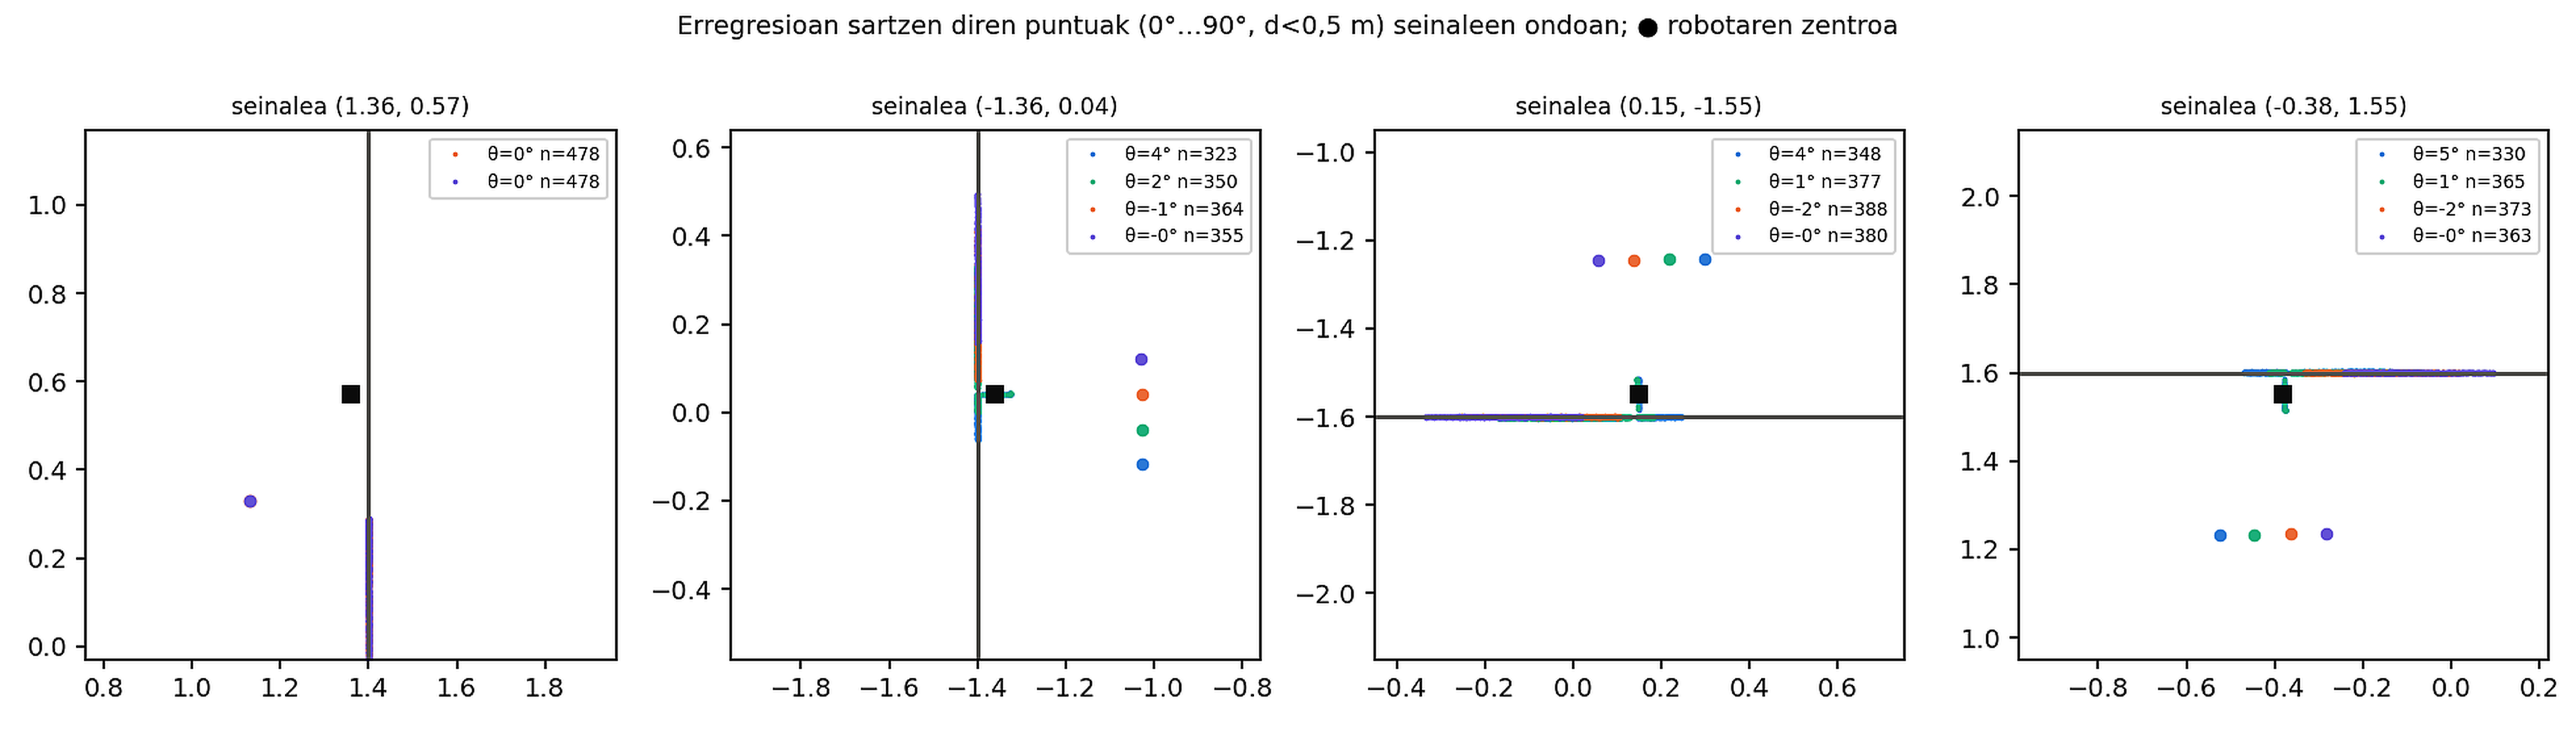
\includegraphics[width=\textwidth]{diag_kp2.png}
\caption{Laser-puntuak eta doitutako zuzena seinale baten ondoan ($K_p = 2{,}0$).}\label{fig:diag-kp2}
\end{figure}

\clearpage
\section[Kontrol Proportzionala]{Kontrol Proportzionalaren emaitzak}\label{sec:emaitzak-p}
\noindent\textit{Enuntziatuko galdera: Kpren zein balio tartean da portaera egokia?}\par\vspace{1pt}

$K_p$-ren eragina aztertzeko, gainerako parametroak finko mantendu ditugu: $K_i = 0$, $K_d = 0$, $v_0 = 0{,}2\text{ m/s}$ eta $K_V = 0$. Konfigurazio bakoitzarekin hiru buelta osatzen saiatu gara (\ref{tab:kp-sweep} taula). Taulako $d$ balioa robotaren zentrotik kanpoko paretarainoko batez besteko distantzia da zuzenetan; $\pm$ ikurrak distantzia horren desbideratze estandarra adierazten du. $\theta_{\text{RMS}}$ balioak, berriz, angelu-errorearen batez besteko tamaina laburbiltzen du: balioa zenbat eta txikiagoa izan, orduan eta paraleloago joan da robota.

\begin{table}[H]
\centering\footnotesize
\renewcommand{\arraystretch}{0.92}
\begin{tabularx}{\textwidth}{@{} l >{\raggedright\arraybackslash}X c c >{\centering\arraybackslash}p{2.6cm} >{\centering\arraybackslash}p{2.3cm} @{}}
\toprule
\textbf{Proba} & \textbf{Emaitza} & \textbf{Bueltak} & \textbf{Talkak} & \textbf{$d$ zuzenetan [m]} & \textbf{$\theta_{\text{RMS}}$ zuzenetan [$^\circ$]} \\
\midrule
$K_p = 0{,}3$ & Pareta galtzen du & $0{,}77$ & $4$  & $0{,}160 \pm 0{,}065$ & $19{,}7$ \\
$K_p = 0{,}6$ & Bueltak osatu, talkekin & $3{,}32$ & $14$ & $0{,}172 \pm 0{,}060$ & $6{,}8$ \\
$K_p = 1{,}0$ & Bueltak osatu, talkekin & $3{,}32$ & $10$ & $0{,}180 \pm 0{,}047$ & $3{,}4$ \\
$K_p = 1{,}5$ & Ondo (optimoa)          & $3{,}32$ & $0$  & $0{,}307 \pm 0{,}013$ & $1{,}7$ \\
$K_p = 2{,}0$ & Ondo                    & $3{,}32$ & $0$  & $0{,}362 \pm 0{,}028$ & $1{,}7$ \\
$K_p = 2{,}5$ & Bueltak osatu, talkekin & $3{,}21$ & $7$  & $0{,}502 \pm 0{,}270$ & $14{,}9$ \\
$K_p = 3{,}0$ & Pareta galtzen du       & $0{,}60$ & $10$ & $0{,}621 \pm 0{,}295$ & $32{,}5$ \\
$K_p = 4{,}0$ & Pareta galtzen du       & $0{,}83$ & $7$  & $0{,}551 \pm 0{,}225$ & $32{,}9$ \\
$K_p = 8{,}0$ & Pareta galtzen du       & $0{,}01$ & $1$  & $0{,}185 \pm 0{,}098$ & $14{,}3$ \\
\bottomrule
\end{tabularx}
\caption{$K_p$ parametroaren eragina abiadura konstantearekin.}\label{tab:kp-sweep}
\end{table}

Probatutako balioen artean, portaera egokia $K_p = 1{,}5$ eta $K_p = 2{,}0$ balioekin lortu dugu: biek osatu dute ibilbidea kontakturik gabe. Emaitza horrek probatutako balioei buruz hitz egiten du; tarteko balio guztiak ez ditugu banan-banan egiaztatu.

\vspace{0.3em}
\noindent\textit{Enuntziatuko galdera: Zein da Kp handitzeak/txikitzeak duen eragina robotak irudikatzen duen bidean? Zergatik?}\par\vspace{1pt}

$K_p$ txikiekin robotak berandu zuzentzen du norabidea. Horregatik, $K_p = 0{,}6$ eta $K_p = 1{,}0$ balioekin kurbak zabalegi hartu eta paretako seinaleak jo ditu. $K_p$ handitzean zuzenketa azkarragoa da, baina gehiegizko balioek kontrako arazoa sortzen dute: robotak gehiegi biratzen du, oszilatzen hasten da eta LiDAR-aren eremutik pareta galtzen du. $K_p = 2{,}5$ balioarekin hiru buelta baino gehiago osatu ditu, baina zazpi kontakturekin; $K_p \ge 3{,}0$ balioekin ez du buelta osoa osatu.

\clearpage
\noindent\textit{Enuntziatuko galdera: Jaso robotaren posizioa denboran zehar eta irudikatu jarraitutako ibilbideak Kp balio desberdinetarako. Irudikatu ere, beste grafika batean, paretarekiko angelua denboran zehar:}\par\vspace{1pt}

\begin{figure}[H]
\centering
\begin{subfigure}[b]{0.48\textwidth}
  \centering
  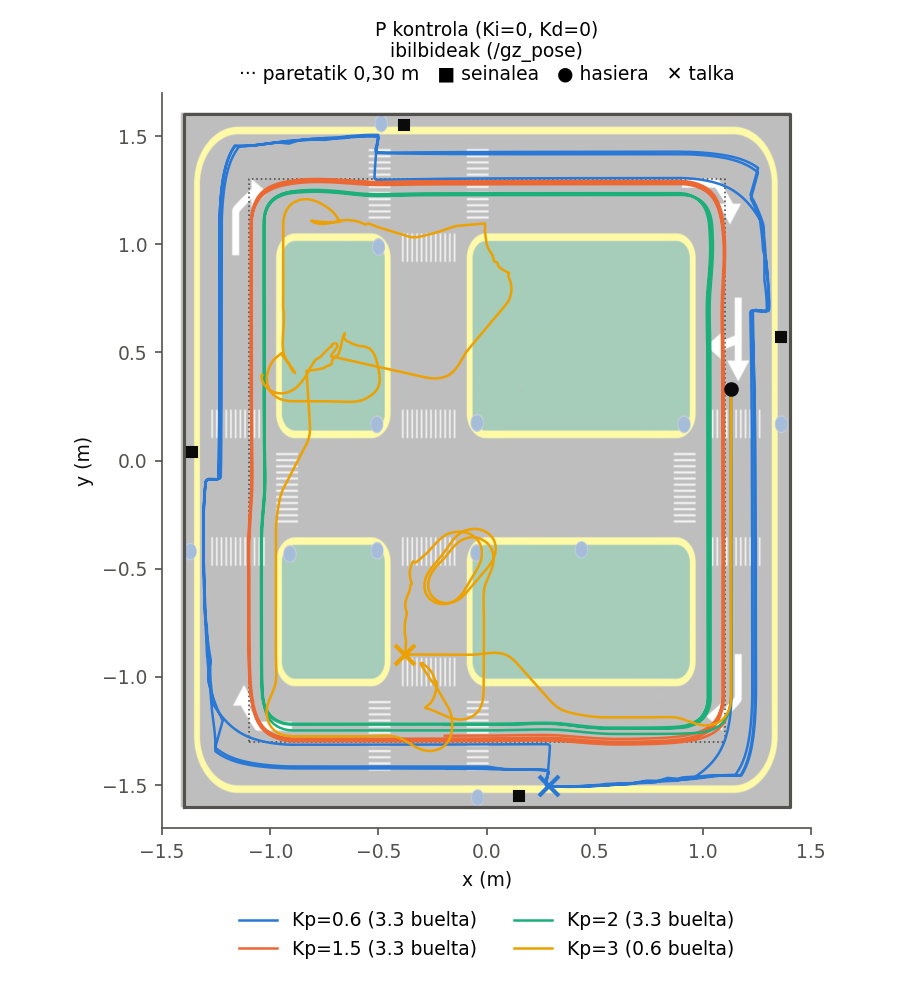
\includegraphics[height=7.2cm, keepaspectratio]{kp_ibilbideak.png}
  \caption{Ibilbideak zirkuituan (\texttt{/gz\_pose}).}\label{fig:kp-ibilbideak}
\end{subfigure}
\hfill
\begin{subfigure}[b]{0.48\textwidth}
  \centering
  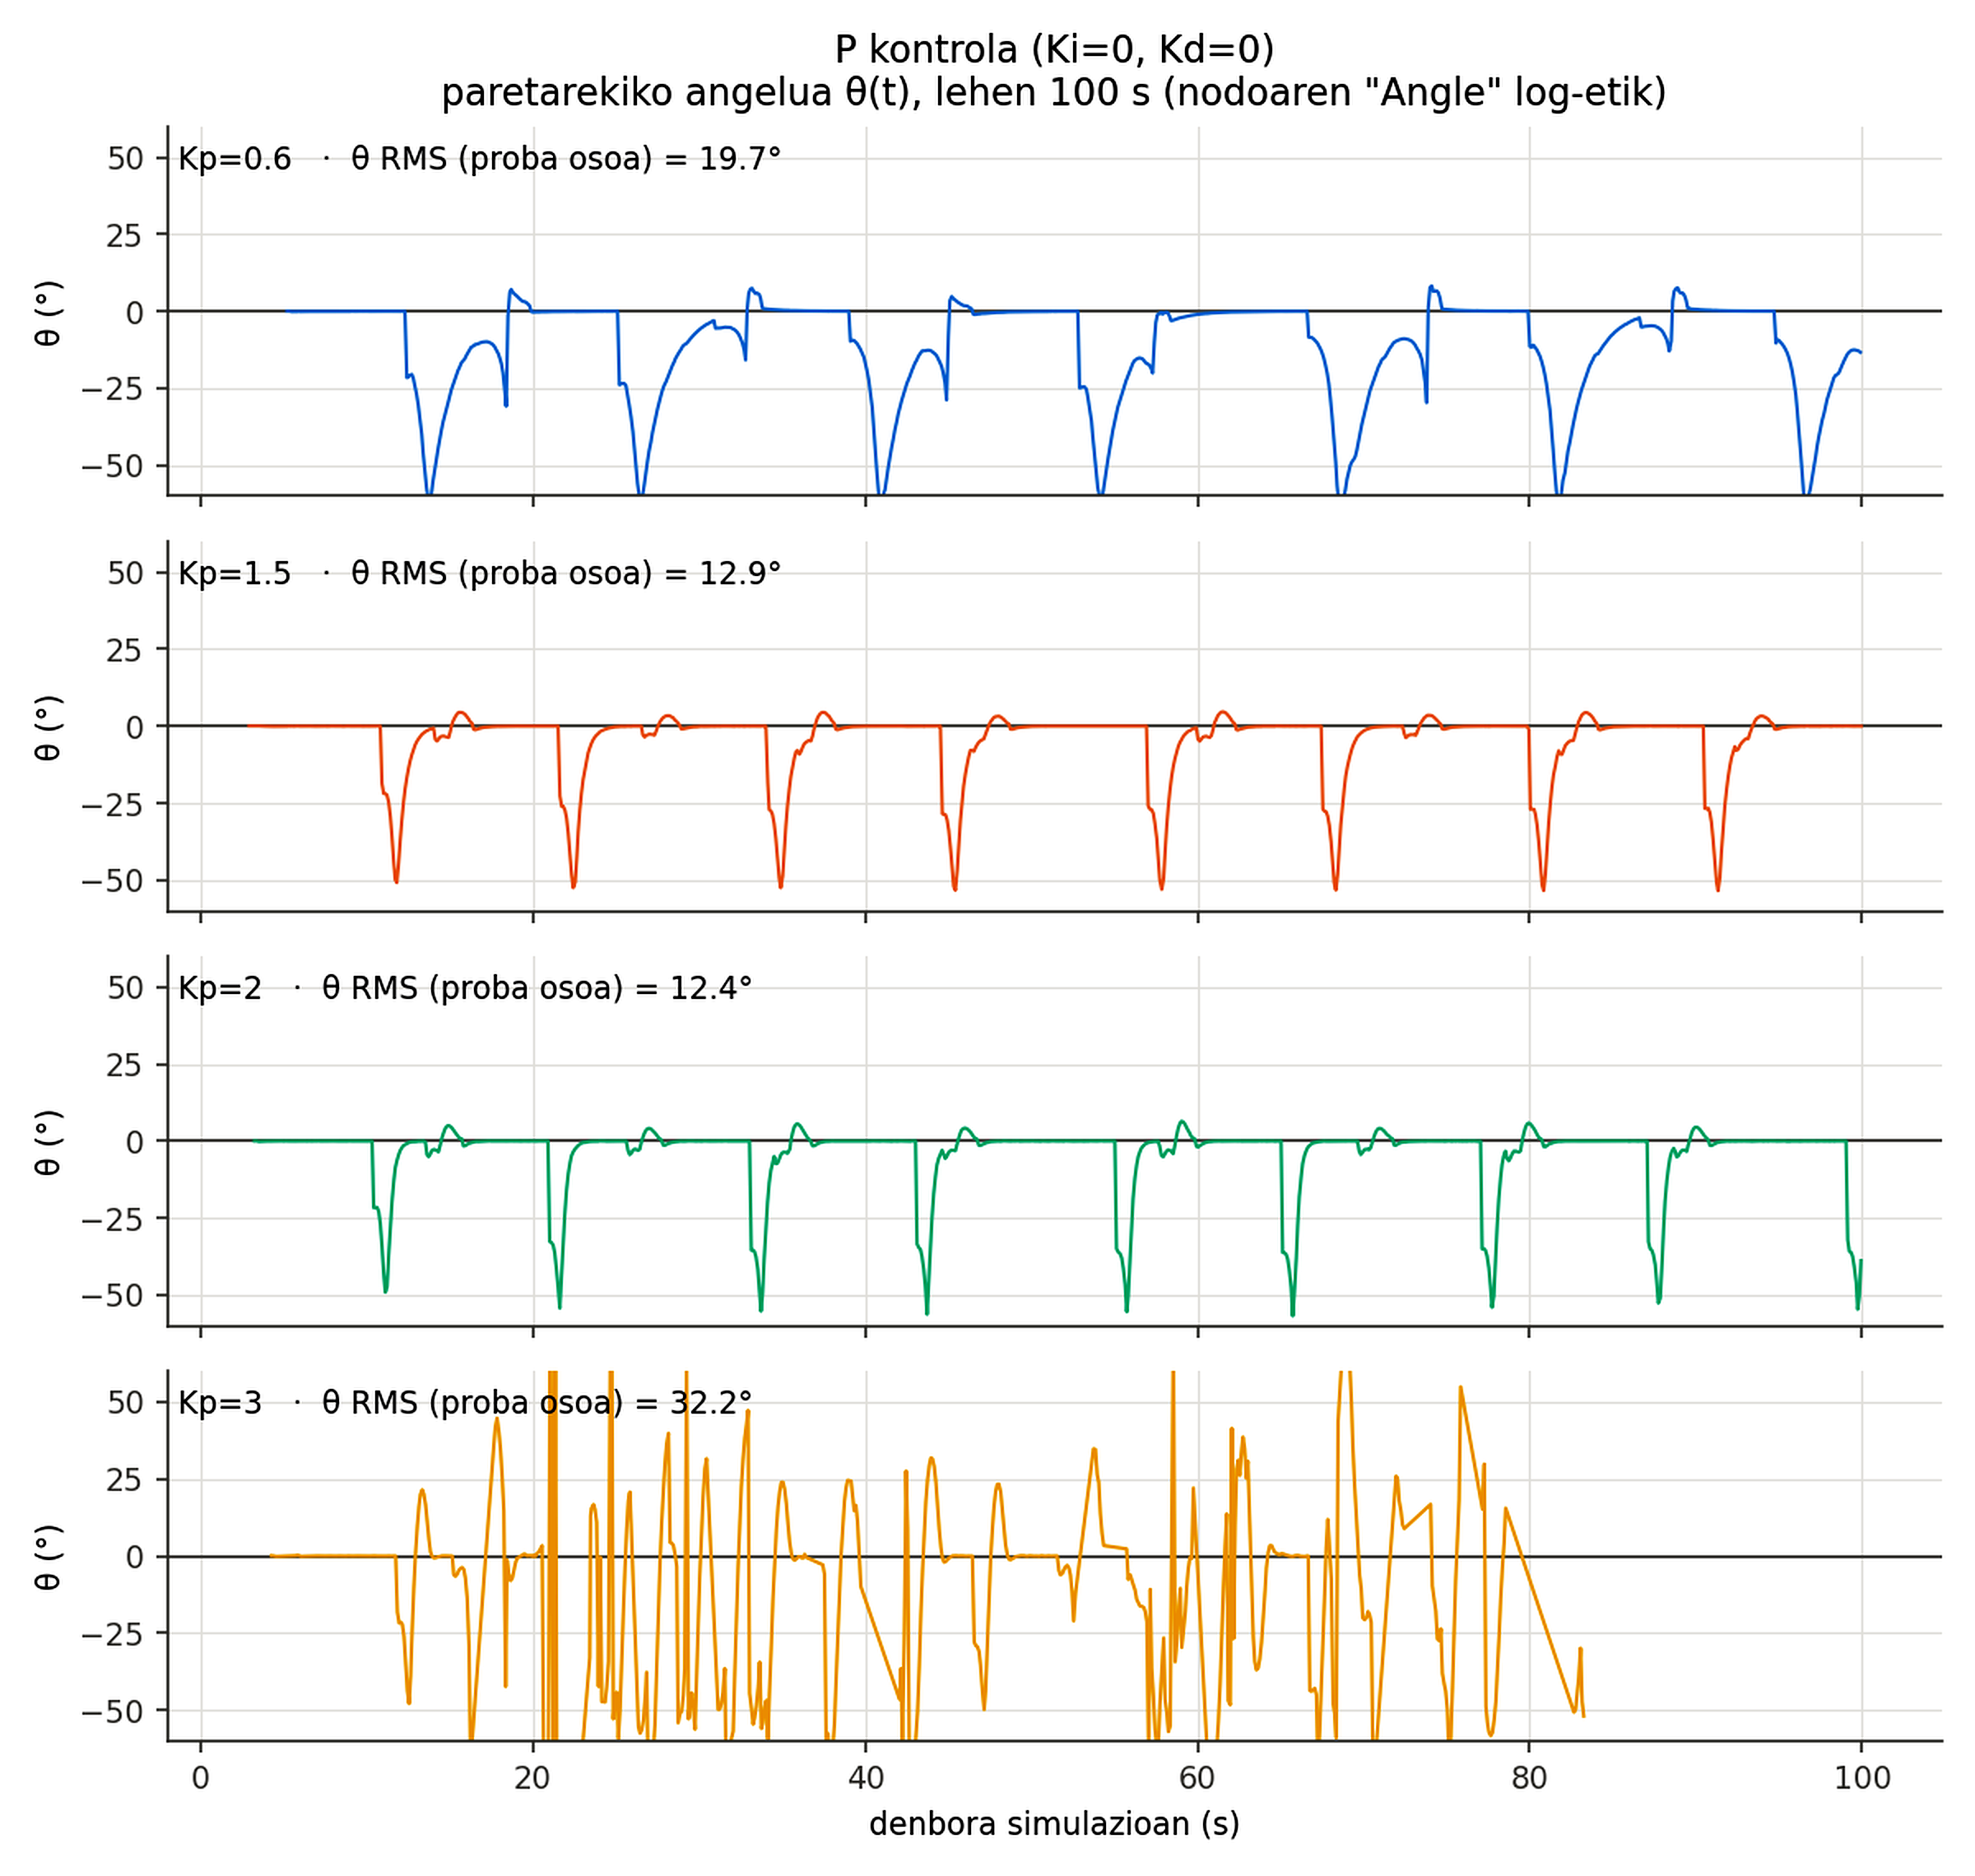
\includegraphics[height=7.2cm, keepaspectratio]{kp_angeluak.png}
  \caption{$\theta$ angelua denboran zehar.}\label{fig:kp-angeluak}
\end{subfigure}
\caption{$K_p$ parametroaren eragina ibilbidean eta paretarekiko angeluan.}\label{fig:kp-grafikoak}
\end{figure}

\ref{fig:kp-grafikoak} irudian ikusten denez, ibilbideek taulako ondorioa berresten dute. $K_p$ txikiekin robota kanpoko paretara hurbiltzen da kurbetan; $K_p$ handiekin, berriz, ibilbidea ezegonkor bihurtzen da. $K_p = 1{,}5$ eta $K_p = 2{,}0$ balioekin ibilbidea erregularra da eta zuzenetako $\theta_{\text{RMS}}$ $1{,}7^\circ$-koa izan da.

\clearpage
\section[Abiadura lineala]{Abiadura linealaren eragina}\label{sec:emaitzak-abiadura}
\noindent\textit{Enuntziatuko galdera: Abiadura linealaren kasuan, abiadura konstante batekin eta alderantziz proportzionalarekin probatu.}\par\vspace{1pt}

Enuntziatuak abiadura konstantea eta biraketaren alderantziz proportzionala den abiadura alderatzeko eskatzen du. Horregatik, $K_V = 0$ eta $K_V = 2$ probatu ditugu $K_p$-ren hainbat baliorekin (\ref{tab:abiadura-sweep} taula eta \ref{fig:v-ibilbideak} irudia). $K_V = 2$ denean robota moteldu egiten da kurbetan, eta horrek biraketa bakoitzean aurreratzen duen distantzia murrizten du.

\begin{table}[H]
\centering\footnotesize
\begin{tabularx}{\textwidth}{@{} l >{\raggedright\arraybackslash}X c c >{\centering\arraybackslash}p{2.6cm} >{\centering\arraybackslash}p{2.3cm} @{}}
\toprule
\textbf{Konfigurazioa} & \textbf{Emaitza} & \textbf{Bueltak} & \textbf{Talkak} & \textbf{$d$ zuzenetan [m]} & \textbf{$\theta_{\text{RMS}}$ zuzenetan [$^\circ$]} \\
\midrule
$K_p = 0{,}6, K_V = 0$ & Talkak seinaleetan & $3{,}32$ & $14$ & $0{,}172 \pm 0{,}060$ & $6{,}8$ \\
$K_p = 0{,}6, K_V = 2$ & Talkak seinaleetan & $3{,}24$ & $14$ & $0{,}166 \pm 0{,}050$ & $7{,}0$ \\
$K_p = 1{,}0, K_V = 0$ & Talkak seinaleetan & $3{,}32$ & $10$ & $0{,}180 \pm 0{,}047$ & $3{,}4$ \\
$K_p = 1{,}0, K_V = 2$ & Ondo (lagundu)     & $3{,}32$ & $0$  & $0{,}384 \pm 0{,}037$ & $2{,}6$ \\
$K_p = 1{,}5, K_V = 0$ & Ondo (optimoa)     & $3{,}32$ & $0$  & $0{,}307 \pm 0{,}013$ & $1{,}7$ \\
$K_p = 1{,}5, K_V = 2$ & Pareta galtzen du  & $0{,}20$ & $4$  & $0{,}646 \pm 0{,}340$ & $26{,}1$ \\
$K_p = 2{,}0, K_V = 0$ & Ondo               & $3{,}32$ & $0$  & $0{,}362 \pm 0{,}028$ & $1{,}7$ \\
$K_p = 2{,}0, K_V = 2$ & Pareta galtzen du  & $0{,}83$ & $3$  & $0{,}674 \pm 0{,}328$ & $32{,}4$ \\
\bottomrule
\end{tabularx}
\caption{Abiadura konstantearen eta kurbetan moteldutako abiaduraren konparaketa.}\label{tab:abiadura-sweep}
\end{table}

Moteltzeak $K_p = 1{,}0$ balioari lagundu dio: kontaktuak 10etik 0ra jaitsi dira. $K_p = 1{,}5$ eta $K_p = 2{,}0$ balioekin, ordea, moteltzeak biraketa gehiegi ixtea eragin du eta robotak pareta galdu du. Beraz, aukeratutako $K_p = 1{,}5$ balioarekin abiadura konstanteak eman du emaitzarik egonkorrena.

\begin{figure}[H]
\centering
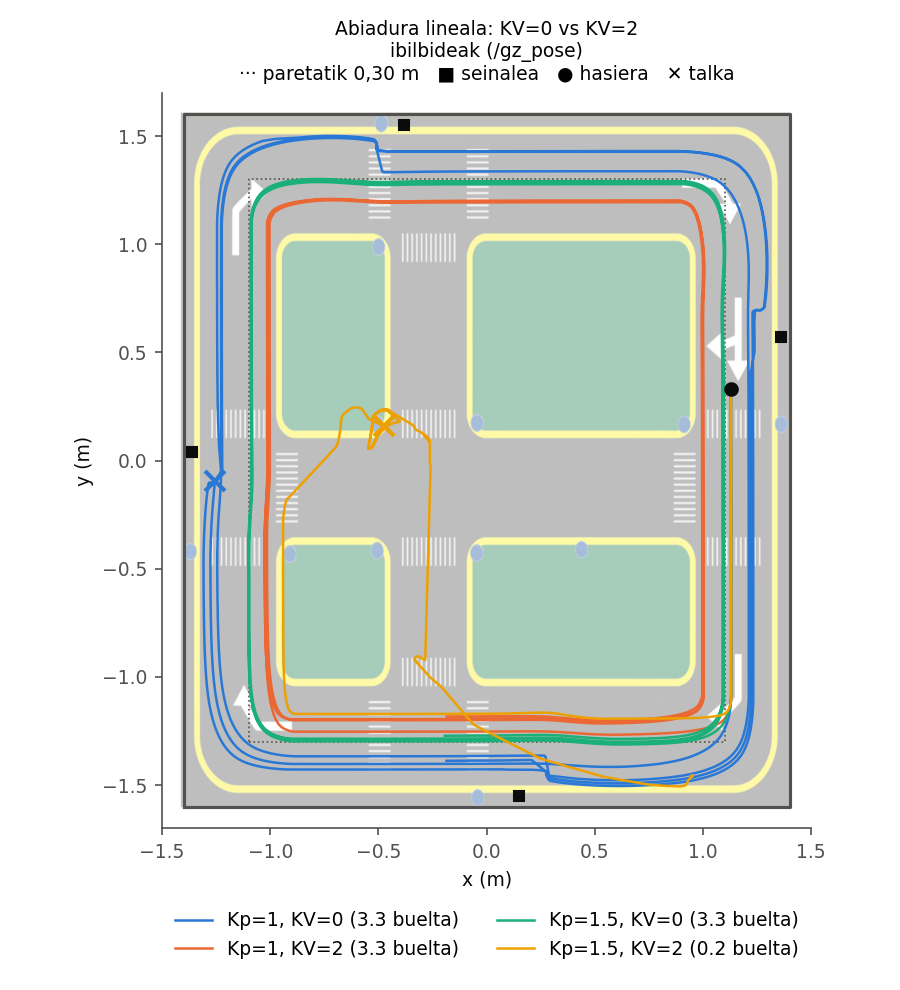
\includegraphics[height=6.8cm, keepaspectratio]{v_ibilbideak.png}
\caption{$K_V = 0$ eta $K_V = 2$ abiadura-legeekin lortutako ibilbideak.}\label{fig:v-ibilbideak}
\end{figure}

\clearpage
\section[PID kontrola]{PID kontrolaren emaitzak (Ki eta Kd)}\label{sec:emaitzak-pid}
\noindent\textit{Enuntziatuko galdera: Aurreko ataletik datorren Kpren abiapuntu on bat hartuta, Ki eta Kdren zein balio tartean da portaera egokia?}\par\vspace{1pt}

$K_p = 2{,}0$ hartu dugu abiapuntutzat, P kontrolarekin kontakturik gabe amaitu duelako eta zuzenetako $\theta_{\text{RMS}}$ $1{,}7^\circ$ izan delako. Ondoren, $K_i$ eta $K_d$ banan-banan aldatu ditugu, osagai bakoitzaren eragina bestearekin nahastu gabe ikusteko (\ref{tab:pid-sweep} taula). Probatutakoen artean, portaera egokia $K_i = 0\dots0{,}2$ tartean eta $K_d = 0{,}05\dots0{,}3$ tartean lortu dugu. Hala ere, tarte horietako balio guztiak ez ditugu probatu: taulan agertzen diren balio zehatzak egiaztatu ditugu.

\begin{table}[H]
\centering\footnotesize
\begin{tabularx}{\textwidth}{@{} l >{\raggedright\arraybackslash}X c c >{\centering\arraybackslash}p{2.6cm} >{\centering\arraybackslash}p{2.3cm} @{}}
\toprule
\textbf{Konfigurazioa} & \textbf{Emaitza} & \textbf{Bueltak} & \textbf{Talkak} & \textbf{$d$ zuzenetan [m]} & \textbf{$\theta_{\text{RMS}}$ zuzenetan [$^\circ$]} \\
\midrule
\multicolumn{6}{l}{\textit{$K_i$ osagaiaren aldaketa ($K_p = 2{,}0, K_d = 0$)}} \\
$K_i = 0{,}0$  & Ondo                    & $3{,}32$ & $0$ & $0{,}362 \pm 0{,}028$ & $1{,}7$ \\
$K_i = 0{,}05$ & Ondo                    & $3{,}32$ & $0$ & $0{,}373 \pm 0{,}033$ & $1{,}7$ \\
$K_i = 0{,}2$  & Ondo                    & $3{,}32$ & $0$ & $0{,}393 \pm 0{,}046$ & $2{,}5$ \\
$K_i = 0{,}5$  & Pareta galtzen du unez  & $3{,}32$ & $4$ & $0{,}443 \pm 0{,}248$ & $14{,}3$ \\
$K_i = 1{,}0$  & Pareta galtzen du       & $0{,}66$ & $2$ & $0{,}542 \pm 0{,}228$ & $38{,}8$ \\
\midrule
\multicolumn{6}{l}{\textit{$K_d$ osagaiaren aldaketa ($K_p = 2{,}0, K_i = 0$)}} \\
$K_d = 0{,}05$ & Ondo              & $3{,}32$ & $0$ & $0{,}362 \pm 0{,}031$ & $1{,}7$ \\
$K_d = 0{,}1$  & Ondo              & $3{,}32$ & $0$ & $0{,}368 \pm 0{,}031$ & $1{,}7$ \\
$K_d = 0{,}3$  & Ondo              & $3{,}32$ & $0$ & $0{,}377 \pm 0{,}038$ & $1{,}7$ \\
$K_d = 1{,}0$  & Trabatu egiten da  & $1{,}57$ & $4$ & $0{,}420 \pm 0{,}317$ & $20{,}3$ \\
\midrule
\multicolumn{6}{l}{\textit{PID konbinazio osoa}} \\
PID ($2{,}0/0{,}05/0{,}1$) & Ondo & $3{,}32$ & $0$ & $0{,}372 \pm 0{,}033$ & $1{,}8$ \\
\bottomrule
\end{tabularx}
\caption{$K_i$ eta $K_d$ bananduta aldatzean lortutako emaitzak eta PID konbinazioa ($K_p = 2{,}0$).}\label{tab:pid-sweep}
\end{table}

\noindent\textit{Enuntziatuko galdera: Zein da Ki handitzeak/txikitzeak duen eragina robotak irudikatzen duen bidean? Zergatik?}\par\vspace{1pt}

I osagaiak kurbetako errorea pilatzen du. Zirkuituko kurba guztiak noranzko berekoak direnez, pilatutako ekarpenak robotari eskuinera biratzen jarraitzeko agintzen dio kurba amaitu ondoren ere. $K_i = 0{,}05$ balioarekin angelu-errorea ia ez da aldatu, baina paretarekiko batez besteko distantzia $0{,}362\text{ m}$-tik $0{,}373\text{ m}$-ra igo da. $K_i \ge 0{,}5$ balioekin desbideratzea handiagoa izan da eta robotak pareta galdu du. Anti-windup mugak pilaketa kontrolatzen laguntzen du, baina probatutako I balioek ez dute P kontrolaren emaitza hobetu.

\vspace{0.4em}
\noindent\textit{Enuntziatuko galdera: Zein da Kd handitzeak/txikitzeak duen eragina robotak irudikatzen duen bidean? Zergatik?}\par\vspace{1pt}

D osagaiak errorearen aldaketa azkarrei erantzuten die. $K_d \le 0{,}3$ balioekin, zuzenetako angelu-errorea P kontrolaren antzekoa izan da, eta ez dugu hobekuntza neurgarririk ikusi. $K_d = 1{,}0$ balioarekin, aldiz, kurbetan paretaren puntu berriak bat-batean sartzeak $\theta$-ren aldaketa handiak sortu ditu. Deribatuak aldaketa horiek handitu ditu eta robotak biraketa-kolpe bortitzak egin eta trabatu egin da.

\clearpage
\noindent\textit{Enuntziatuko galdera: Jaso robotaren posizioa denboran zehar eta irudikatu jarraitutako ibilbideak Kp, Ki eta Kd balio desberdinetarako. Irudikatu ere, beste grafika batean, paretarekiko angelua denboran zehar:}\par\vspace{1pt}

\begin{figure}[H]
\centering
\begin{subfigure}[b]{0.48\textwidth}
  \centering
  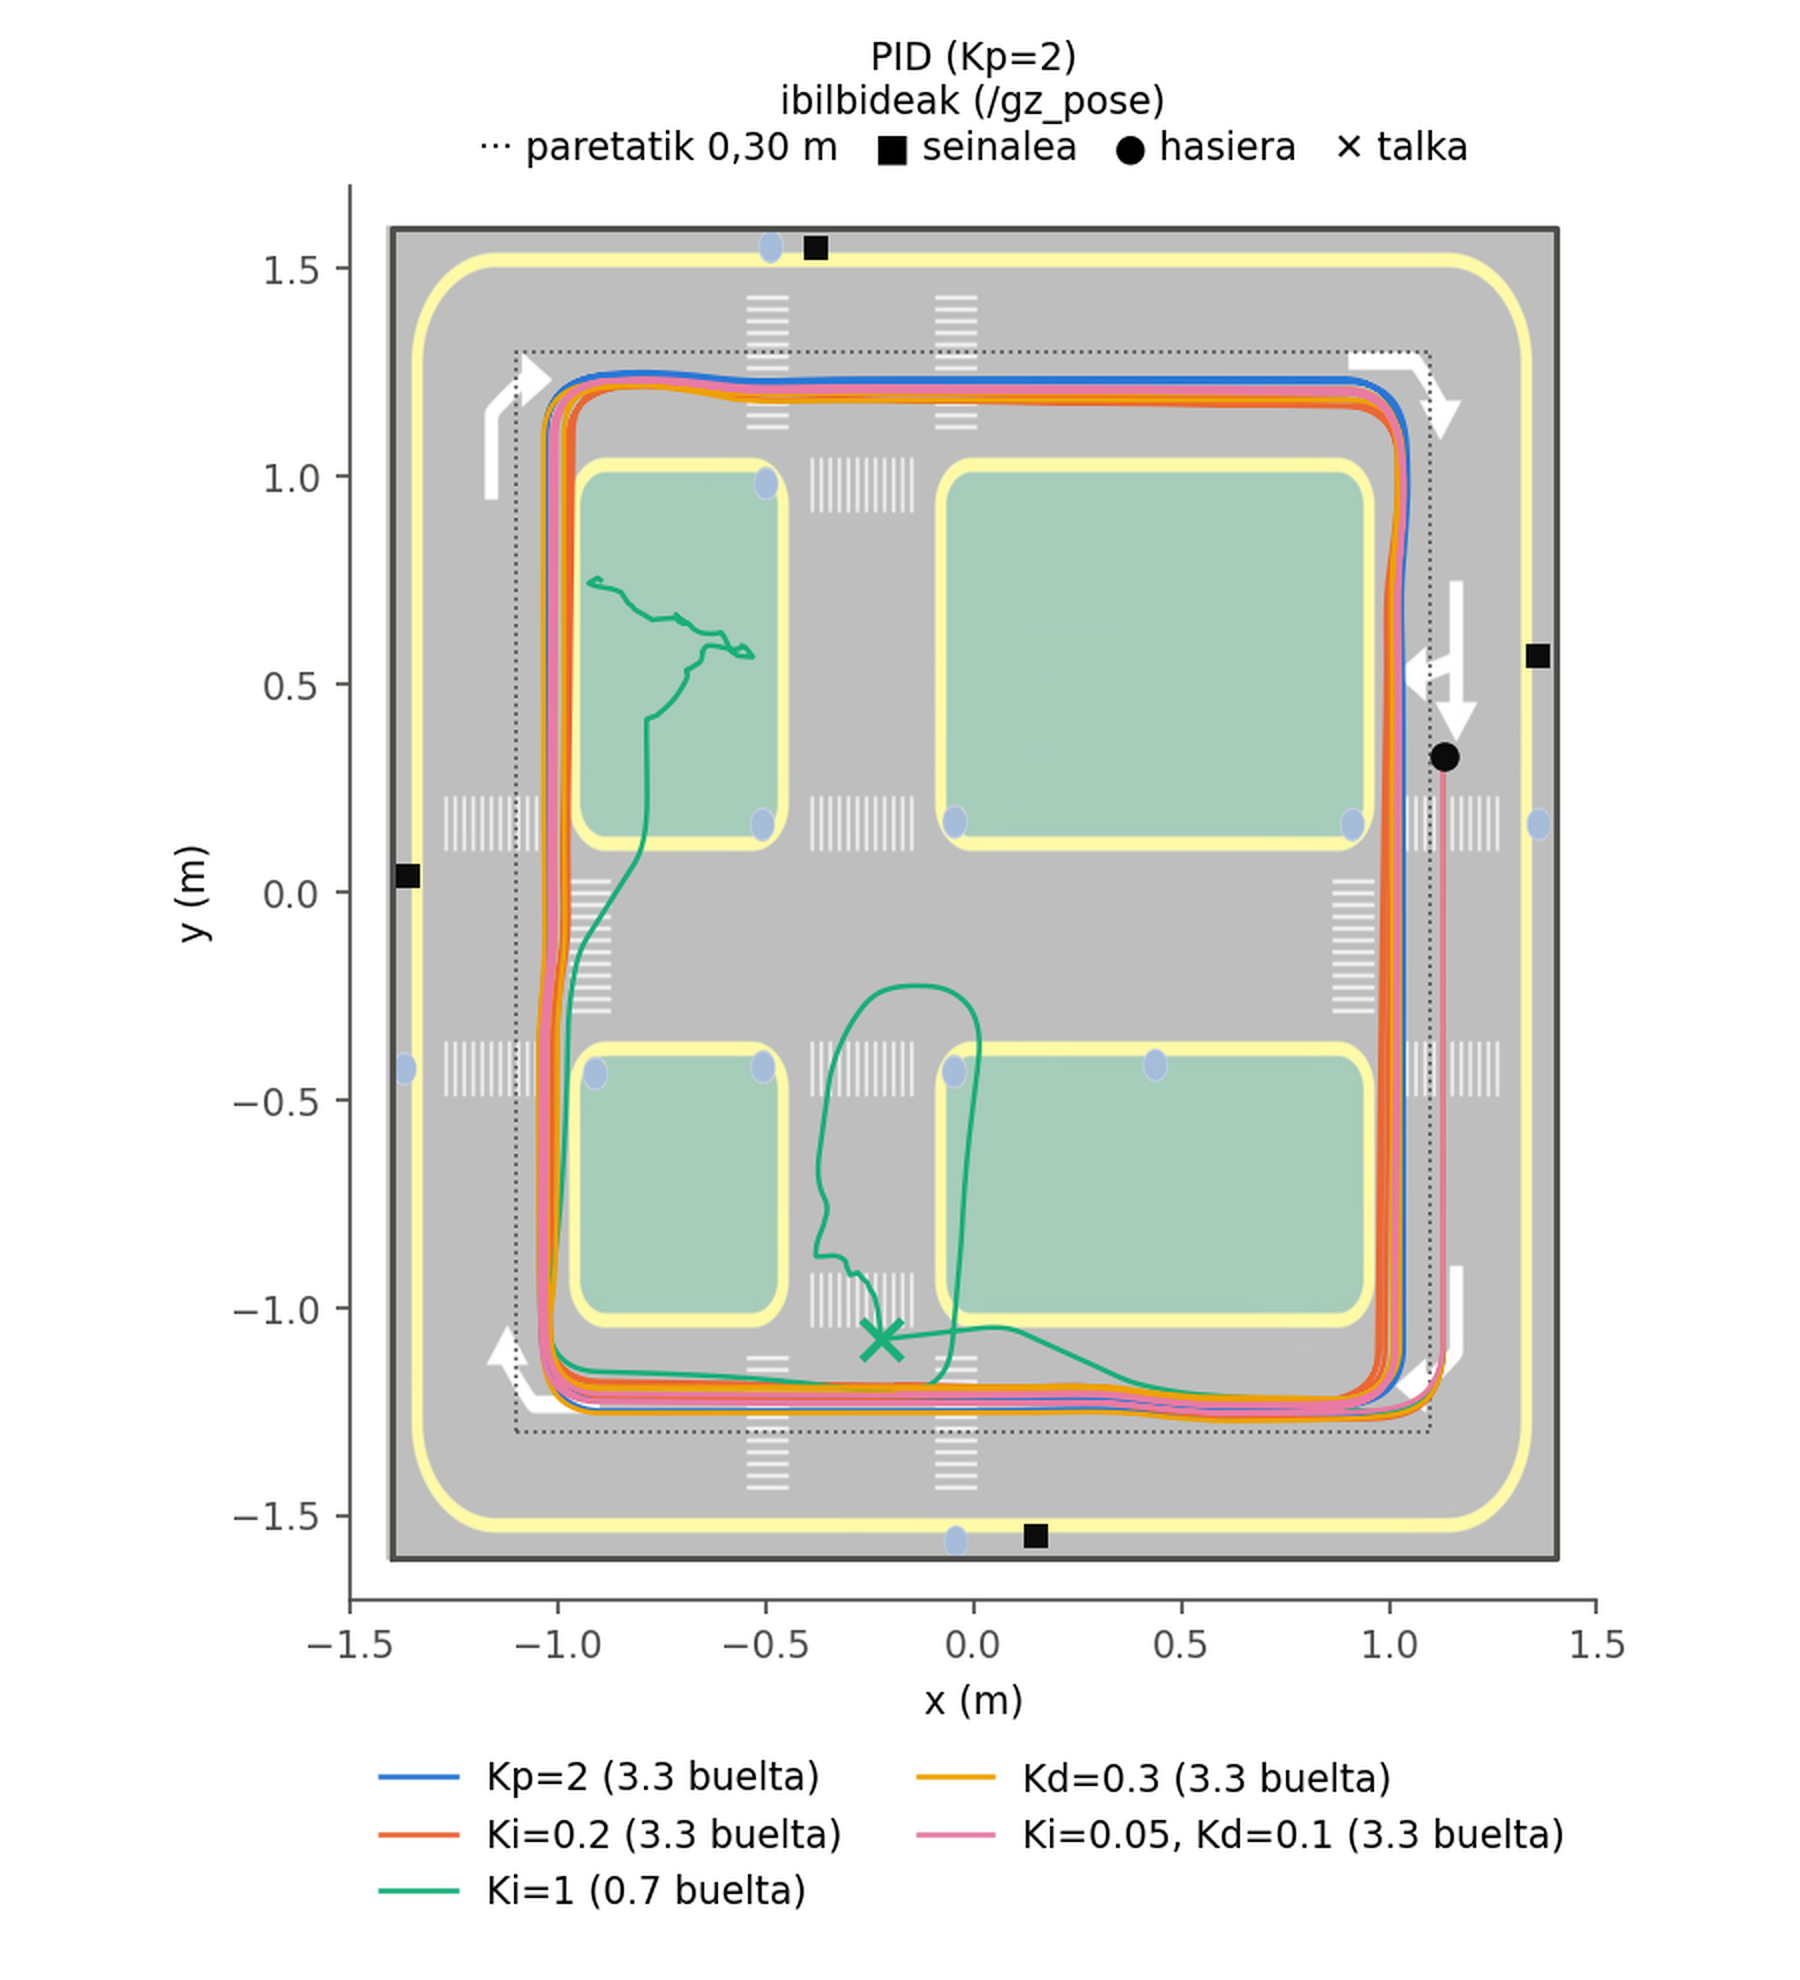
\includegraphics[height=6.0cm, keepaspectratio]{pid_ibilbideak.png}
  \caption{PID ibilbideak.}\label{fig:pid-ibilbideak}
\end{subfigure}
\hfill
\begin{subfigure}[b]{0.48\textwidth}
  \centering
  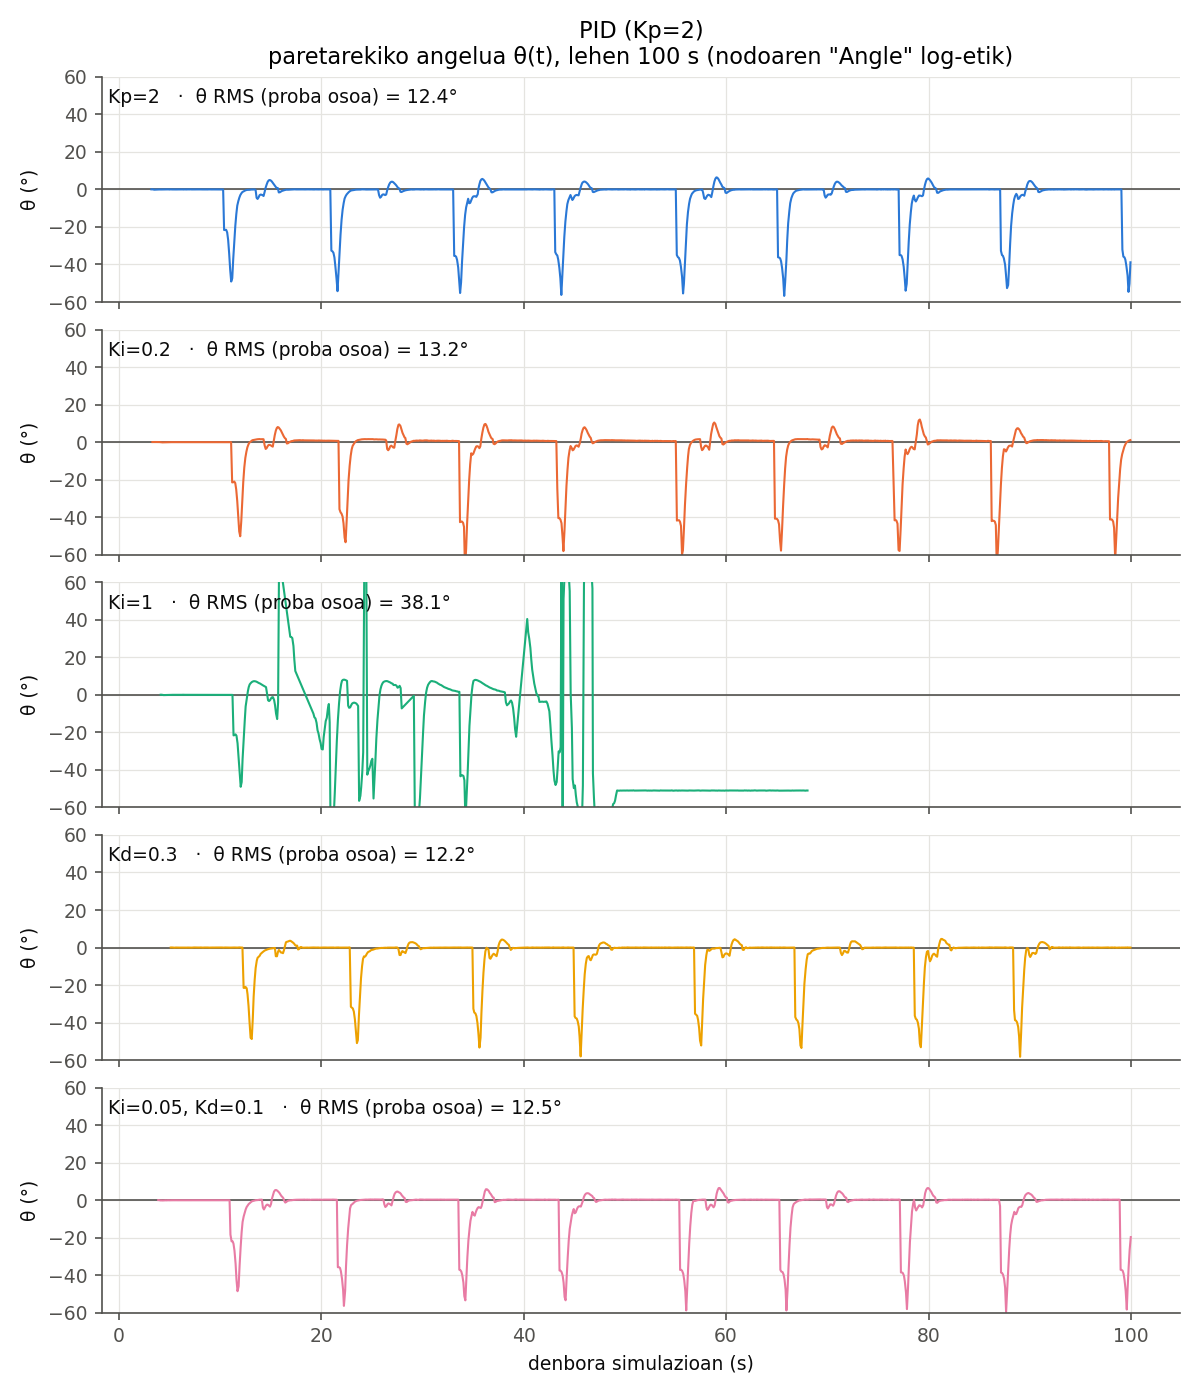
\includegraphics[height=6.0cm, keepaspectratio]{pid_angeluak.png}
  \caption{$\theta$ angelua denboran zehar.}\label{fig:pid-angeluak}
\end{subfigure}
\caption{$K_i$, $K_d$ eta PID konbinazioen eragina ($K_p = 2{,}0$).}\label{fig:pid-grafikoak}
\end{figure}

\ref{fig:pid-grafikoak} irudian ikusten denez, PID konbinazio osoak ($K_p = 2{,}0$, $K_i = 0{,}05$ eta $K_d = 0{,}1$) hiru bueltak kontakturik gabe osatu ditu. Hala ere, $\theta_{\text{RMS}}$ $1{,}8^\circ$ izan da, P hutsaren $1{,}7^\circ$-ren oso antzekoa. Beraz, proba honetan I eta D gehitzeak ez du hobekuntza neurgarririk ekarri.

\clearpage
\section[Enuntziatuko adibideak]{Enuntziatuko hasierako adibideak ($K_p = 0{,}6$)}\label{sec:emaitzak-enuntziatua}
Enuntziatuan hasierako proba gisa emandako hiru konfigurazioak ere exekutatu ditugu (\ref{tab:enuntziatua-sweep} taula eta \ref{fig:enun-ibilbideak} irudia). Hirurek $K_p = 0{,}6$ erabiltzen dute; balio horrekin robotak berandu biratzen du eta kanpoko seinaleak jotzen ditu. $K_i$ edo $K_d$ gehitzeak ez du arazo hori konpondu probatutako konfigurazioetan.

\begin{table}[H]
\centering\footnotesize
\begin{tabularx}{\textwidth}{@{} >{\raggedright\arraybackslash}p{2.3cm} >{\raggedright\arraybackslash}X c c >{\centering\arraybackslash}p{2.5cm} >{\centering\arraybackslash}p{2.2cm} @{}}
\toprule
\textbf{Agindua} & \textbf{Emaitza} & \textbf{Bueltak} & \textbf{Talkak} & \textbf{$d$ zuzenetan [m]} & \textbf{$\theta_{\text{RMS}}$ zuzenetan [$^\circ$]} \\
\midrule
\texttt{kp:=0.6}\newline \texttt{ki:=0.0}\newline \texttt{kd:=0.0} & Talkak seinaleetan & $3{,}32$ & $14$ & $0{,}172 \pm 0{,}060$ & $6{,}8$ \\
\addlinespace[0.2em]
\texttt{kp:=0.6}\newline \texttt{ki:=0.05}\newline \texttt{kd:=0.0} & Talkak seinaleetan & $3{,}32$ & $13$ & $0{,}167 \pm 0{,}048$ & $6{,}9$ \\
\addlinespace[0.2em]
\texttt{kp:=0.6}\newline \texttt{ki:=0.05}\newline \texttt{kd:=0.1} & Talkak seinaleetan & $3{,}32$ & $13$ & $0{,}189 \pm 0{,}069$ & $7{,}0$ \\
\bottomrule
\end{tabularx}
\caption{Enuntziatuko hasierako konfigurazioen emaitzak.}\label{tab:enuntziatua-sweep}
\end{table}

\begin{figure}[H]
\centering
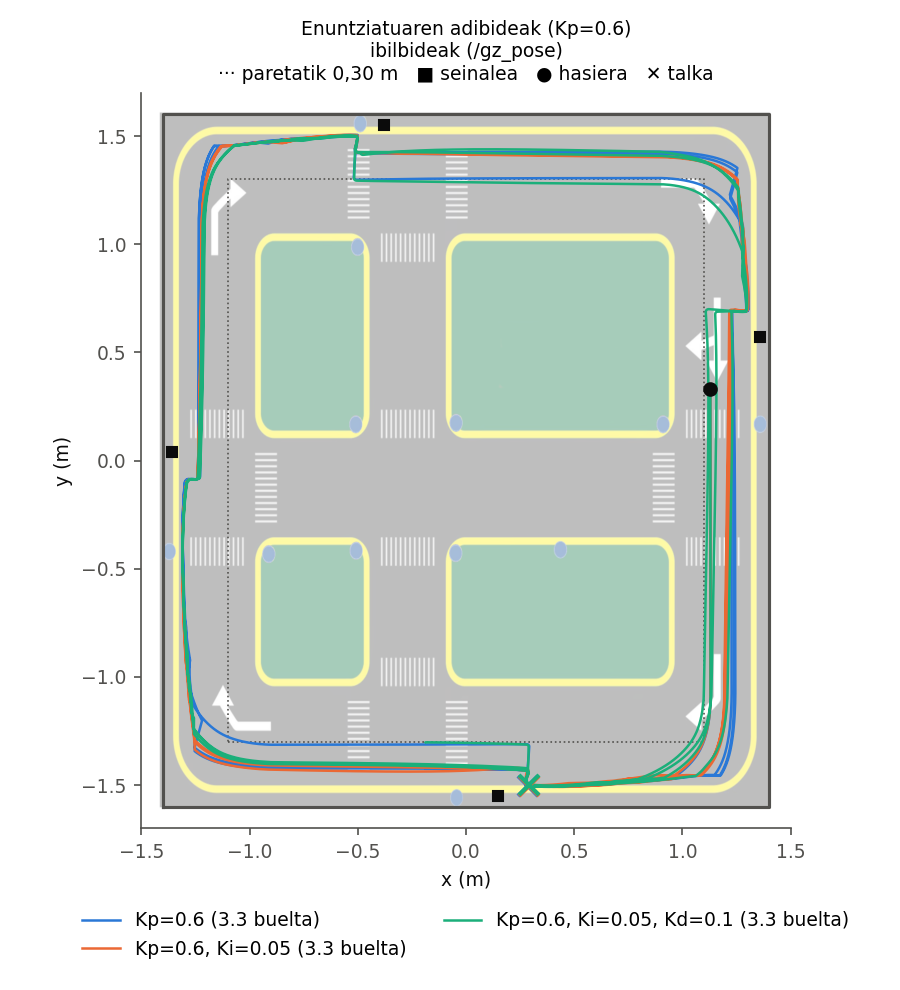
\includegraphics[height=7.5cm, keepaspectratio]{enun_ibilbideak.png}
\caption{Enuntziatuko hiru konfigurazioekin lortutako ibilbideak.}\label{fig:enun-ibilbideak}
\end{figure}
